\documentclass[11pt,a4paper]{article}
\usepackage[utf8]{inputenc}
\usepackage[T1]{fontenc}
\usepackage{lmodern}
\usepackage[margin=2.2cm]{geometry}
\usepackage{amsmath,amssymb}
\usepackage{graphicx}
\usepackage{booktabs}
\usepackage{siunitx}
\usepackage{caption}
\usepackage{subcaption}
\usepackage{float}
\usepackage{xcolor}
\usepackage{listings}
\usepackage[hidelinks]{hyperref}

\graphicspath{{../plot/}}
\setlength{\emergencystretch}{2em}
\makeatletter\newcommand{\rowsinput}[1]{\@@input #1 }\makeatother
\sisetup{detect-all, group-separator={\,}, group-minimum-digits=5}
\captionsetup{font=small,labelfont=bf}
\lstset{basicstyle=\ttfamily\footnotesize, basewidth=0.5em, columns=fixed, keepspaces=true, frame=single,
        breaklines=true, keywordstyle=\color{blue!60!black}}

\newcommand{\KcChapter}{3230.3}
\newcommand{\KcRef}{3213}
\newcommand{\VcRef}{90.5}
\newcommand{\PcRef}{969}
\newcommand{\FcRef}{643}
\newcommand{\KcDevMax}{0.5}
\newcommand{\PcErrOneMin}{6.6}
\newcommand{\PcErrOneMax}{8.8}
\newcommand{\PcErrTwoMin}{0.6}
\newcommand{\PcErrTwoMax}{7.6}
\newcommand{\PcTwoPredFirst}{1867}
\newcommand{\PcTwoPredLast}{974}
\newcommand{\KcOneMean}{3003}
\newcommand{\KcOneStd}{19}
\newcommand{\KcTwoMean}{3100}
\newcommand{\KcTwoStd}{72}
\newcommand{\KcTwoMin}{3003}
\newcommand{\KcTwoMax}{3213}
\newcommand{\KcAllMean}{3052}
\newcommand{\KcRefMin}{3213}
\newcommand{\KcRefMax}{2845}
\newcommand{\KcRangeMin}{2845}
\newcommand{\KcRangeMax}{3284}
\newcommand{\BandOne}{202}
\newcommand{\BandTwo}{368}
\newcommand{\DevMinMax}{11.5}
\newcommand{\KcCrossLo}{736}
\newcommand{\KcCrossHi}{5321}
\newcommand{\SwingCut}{710}
\newcommand{\SwingAir}{756}
\newcommand{\PcOneMean}{1502}
\newcommand{\PcOnePred}{1615}
\newcommand{\PcTwoFirst}{1738}
\newcommand{\PcTwoLast}{969}
\newcommand{\PzeroOneFirst}{347}
\newcommand{\PzeroOneLast}{811}
\newcommand{\PzeroTwoFirst}{474}
\newcommand{\PzeroTwoLast}{419}
\newcommand{\PzeroFitTwelve}{406}
\newcommand{\IdleA}{55}
\newcommand{\IdleB}{0.156}
\newcommand{\IdleC}{1.14}
\newcommand{\TcutOne}{105.6}
\newcommand{\TcutOnePred}{105.6}
\newcommand{\TcutTwo}{119.8}
\newcommand{\TcutTwoPred}{120.0}
\newcommand{\ToneTot}{117.9}
\newcommand{\TtwoTot}{129.1}
\newcommand{\EOne}{210}
\newcommand{\ETwo}{214}
\newcommand{\ECutOne}{159}
\newcommand{\ECutTwo}{163}
\newcommand{\RiseMean}{0.14}
\newcommand{\TonDelayOne}{0.09}
\newcommand{\TonDelayTwo}{0.07}
\newcommand{\SECcutOne}{2.92}
\newcommand{\SECcutTwo}{3.01}

\newcommand{\DrKc}{3213}
\newcommand{\DrKf}{1285}
\newcommand{\DrVc}{90.5}
\newcommand{\DrFiveN}{5760}
\newcommand{\DrFiveVf}{1152}
\newcommand{\DrFiveE}{570}
\newcommand{\DrFiveTZero}{0.052}
\newcommand{\DrFiveZZero}{0.00}
\newcommand{\DrFiveTOne}{0.127}
\newcommand{\DrFiveZOne}{1.44}
\newcommand{\DrFiveTTwo}{0.573}
\newcommand{\DrFiveZTwo}{10.00}
\newcommand{\DrThirteenN}{2215}
\newcommand{\DrThirteenVf}{443}
\newcommand{\DrThirteenE}{6892}
\newcommand{\DrThirteenTZero}{0.331}
\newcommand{\DrThirteenZZero}{1.44}
\newcommand{\DrThirteenTOne}{0.644}
\newcommand{\DrThirteenZOne}{3.75}
\newcommand{\DrThirteenTTwo}{1.490}
\newcommand{\DrThirteenZTwo}{10.00}
\newcommand{\DrThirteenTThree}{2.844}
\newcommand{\DrThirteenZThree}{20.00}


\title{\textbf{Assignment 1 -- Cutting power and specific cutting pressure\\
in turning, prediction of a drilling sequence}\\[4pt]
\large Multi-Agent System for Smart Machining (ECIU micro-module, INSA Toulouse)}
\author{Daniele Trisotto}
\date{\today}

\begin{document}
\maketitle

\begin{abstract}
The cutting power of the two turning programs (constant
cutting speed $V_c=\SI{150}{m/min}$ and constant spindle speed $N=\SI{1200}{rpm}$) is
predicted with the mechanistic model $P_c=K_c f a_p V_c$, using the specific cutting
pressure given by the chapter for the smallest diameter ($K_c=\KcChapter$~MPa). The
prediction is compared with the total spindle power published on GitHub, both in
timing and in curve profile. A Python code then separates, pass by pass, the
steady-state power during cutting from the spindle power without cutting and returns
the specific cutting pressure: on the smallest diameter at constant spindle speed it
gives $K_c=\KcRef$~MPa at $V_c=\VcRef$~m/min. With these two values, the feed force,
cutting power and torque of a drilling sequence (pre-drilling $\varnothing$5 mm, then
drilling $\varnothing$13 mm in the same position) are predicted along time.
\end{abstract}

% ===========================================================================
\section{Context and data}
% ===========================================================================
The data come from the chapter ``Integrating Environmental Impact into Cutting Speed
Decisions in CNC Turning'' (A.\,C.~Araujo, document \emph{Inspiration for your
assignment}) and from its repository \texttt{github.com/annacarlaaraujo/chapter\_2025}.
An AISI~4135 bar is reduced from $D=\SI{48}{mm}$ to \SI{24}{mm} over a length of
\SI{40}{mm} with a DNMG coated carbide insert, in 12 passes with radial depth of cut
$a_p=\SI{1}{mm}$ and feed $f=\SI{0.2}{mm/rev}$. Two CNC programs remove the same volume:
\begin{itemize}
  \item \textbf{Program I}, constant cutting speed (G96), $V_c=\SI{150}{m/min}$: the
        spindle speed grows from 1038 to 1989~rpm as the diameter decreases;
  \item \textbf{Program II}, constant spindle speed (G97), $N=\SI{1200}{rpm}$: the
        cutting speed decreases from 173.4 to 90.5~m/min.
\end{itemize}
Each program was run twice, \emph{with} chip removal and \emph{without} (``air cutting'',
files \texttt{*VIDE.csv}). The Siemens trace records the spindle active power and the
programmed and measured X/Z positions every \SI{9}{ms}. The spindle-speed channel is
empty, so the speed is taken from the program and checked through the measured feed
velocity $V_f=fN$.

Figure~\ref{fig:path} shows the programmed path. Each pass starts at $Z=+\SI{1}{mm}$
(\SI{1}{mm} of air feed before the face of the bar, $Z=0$), feeds to $Z=-\SI{40}{mm}$,
retracts in X, comes back in rapid and plunges to the next diameter. The programmed X is
the finished diameter of the pass. As in the chapter (and in the course slides, where
$N$ is computed on the radius $R_P$ of the tool point), the cutting speed is computed
on X: $V_c=\pi X N/1000$.

\begin{figure}[H]
  \centering
  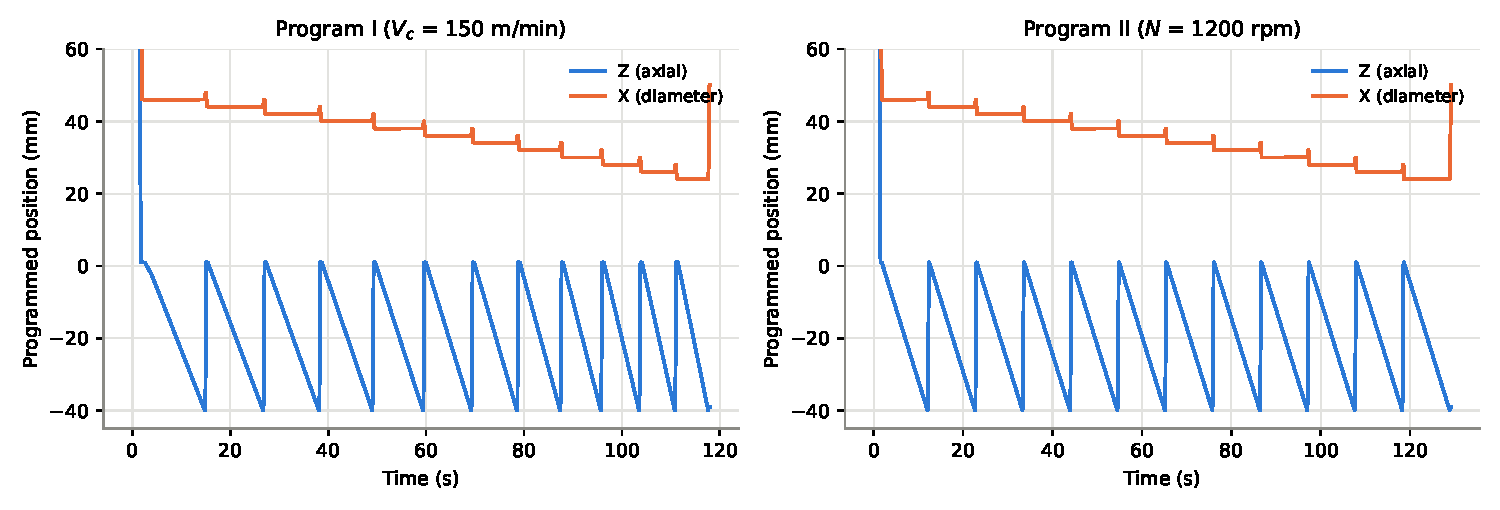
\includegraphics[width=\linewidth]{turning_programmed_path.pdf}
  \caption{Programmed Z and X positions recorded during the cutting runs.}
  \label{fig:path}
\end{figure}

\sloppy
\paragraph{Code.} All computations are done in Python. The code, together with the
input data, is available at
\begin{center}
\url{https://github.com/DanTrisi/MASSMA_1_TOLOSA/tree/master/Assigment1}
\end{center}
Models and signal processing are in \texttt{machining.py}, points 1--3 in
\texttt{turning\_analysis.py} and point 4 in \texttt{drilling\_analysis.py}. Running
\texttt{run\_all.py} produces every figure and every value shown in this report
(Appendix~\ref{app:code}).

% ===========================================================================
\section{Point 1 -- Prediction of the cutting power in turning}
% ===========================================================================
\paragraph{Model.} With the course model (slides ``Power in turning'')
\begin{equation}
  F_c = K_c\, f\, a_p, \qquad
  P_c = F_c\,V_c = K_c\, f\, a_p\, V_c, \qquad
  P_f = K_f\, f\, a_p\, V_f \approx 0 ,
  \label{eq:turning}
\end{equation}
with $K_c$ in MPa, $f\,a_p$ in mm$^2$ and $V_c$ in m/s, $P_c$ is in W. The feed power
is negligible ($V_f$ is about 1000 times smaller than $V_c$).

\paragraph{Parameters.} The specific cutting pressure is the one given by the chapter
(Table~2) for the \emph{smallest diameter}, $X=\SI{24}{mm}$, in Program~2
($N=1200$~rpm): $K_c=\KcChapter$~MPa. It is kept constant for all passes of both
programs. The kinematics come from the program:
\begin{equation}
  N_{I}=\frac{1000\,V_c}{\pi X},\qquad V_{c,II}=\frac{\pi X\cdot 1200}{1000},\qquad
  V_f = f\,N .
\end{equation}

\paragraph{Predicted timings.} For every pass (origin: start of the feed motion at
$Z=+1$~mm):
\begin{itemize}
  \item $t_0$, the tool touches the bar: $t_0 = \SI{1}{mm}/V_f$;
  \item $t_1$, the tool is fully engaged. With an approach angle close to \ang{90}
        the whole depth of cut enters almost at once, and the transition is set by
        the nose radius ($r_\varepsilon=\SI{0.8}{mm}$, assumed): $t_1=t_0+r_\varepsilon/V_f$;
  \item $t_2$, end of the machined length: $t_2=t_0+\SI{40}{mm}/V_f$.
\end{itemize}

\begin{table}[H]
\centering\small
\caption{Point 1: predicted cutting power and timings for each pass
($K_c=\KcChapter$~MPa). Times measured from the start of the feed of the pass.}
\label{tab:pred}
\begin{tabular}{rrrrrrrrr}
\toprule
pass & $X$ (mm) & $N$ (rpm) & $V_c$ (m/min) & $V_f$ (mm/min) & $P_{c,pred}$ (W) &
$t_0$ (s) & $t_1$ (s) & $t_2$ (s)\\
\midrule
\multicolumn{9}{l}{\emph{Program I -- $V_c=150$ m/min}}\\
\rowsinput{../results/prediction_vc150_rows.tex}
\midrule
\multicolumn{9}{l}{\emph{Program II -- $N=1200$ rpm}}\\
\rowsinput{../results/prediction_n1200_rows.tex}
\bottomrule
\end{tabular}
\end{table}

Program~I gives a constant cutting power, $P_c=\PcOnePred$~W, on passes that become
shorter (11.6 to 6.0~s) because $V_f$ grows with $N$. Program~II gives passes of
constant duration (\SI{10}{s} of cut) with a cutting power proportional to the
diameter, decreasing linearly from \PcTwoPredFirst\ to \PcTwoPredLast~W.

% ===========================================================================
\section{Point 2 -- Recorded total power: timings and curve profile}
% ===========================================================================
Figure~\ref{fig:raw} shows the total spindle power recorded on GitHub, with and without
chip removal. The machine does not measure $P_c$ alone: the predicted \emph{total} power
is therefore built as $P_{tot,pred}(t)=P_0+P_c(t)$, where $P_0$ is the spindle power
without cutting identified on the air-cutting run (Section~\ref{sec:kc}) and $P_c(t)$
follows Eq.~\eqref{eq:turning} with a ramp from $t_0$ to $t_1$. It is overlaid on the
measured signal in Fig.~\ref{fig:pred}.

\begin{figure}[H]
  \centering
  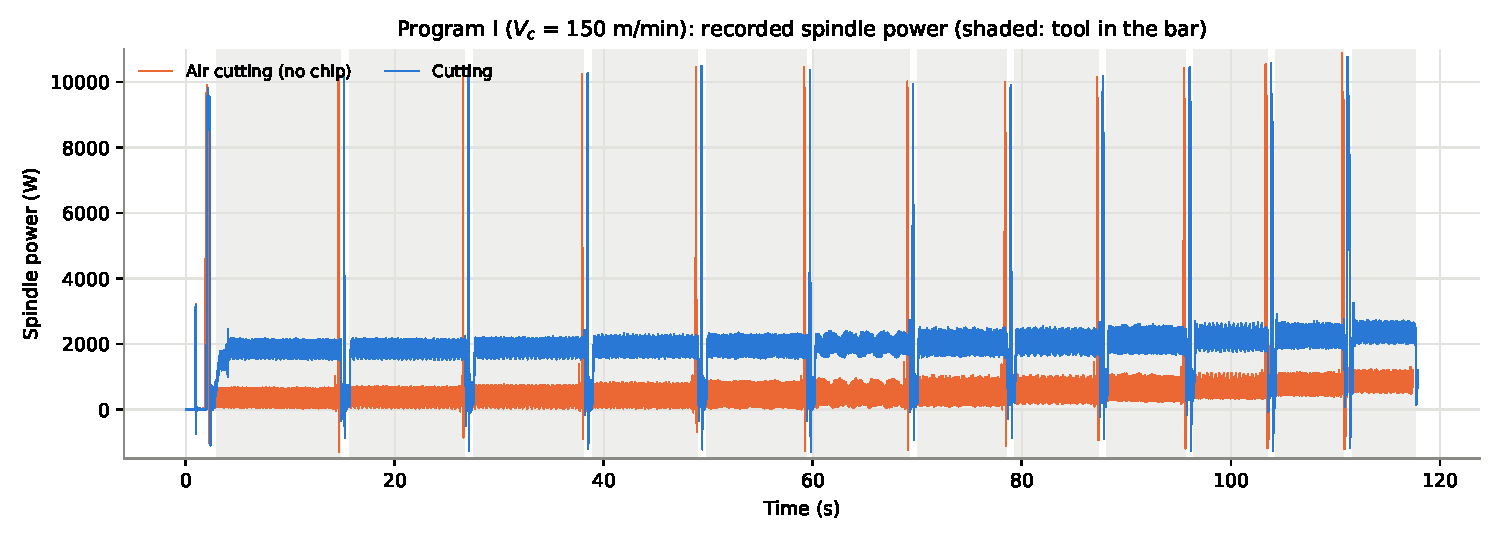
\includegraphics[width=\linewidth]{turning_power_raw_vc150.pdf}\\
  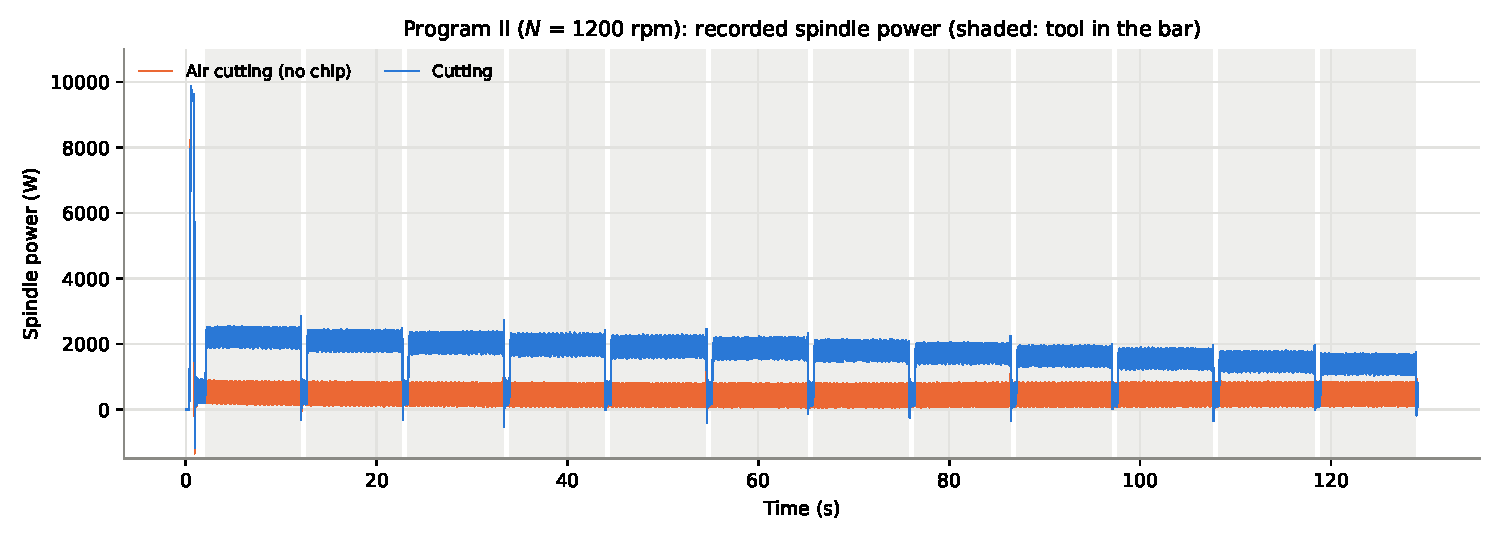
\includegraphics[width=\linewidth]{turning_power_raw_n1200.pdf}
  \caption{Recorded spindle power with chip removal (blue) and without (orange).
  Shaded bands: tool inside the bar ($0\geq Z\geq -40$ mm).}
  \label{fig:raw}
\end{figure}

\begin{figure}[H]
  \centering
  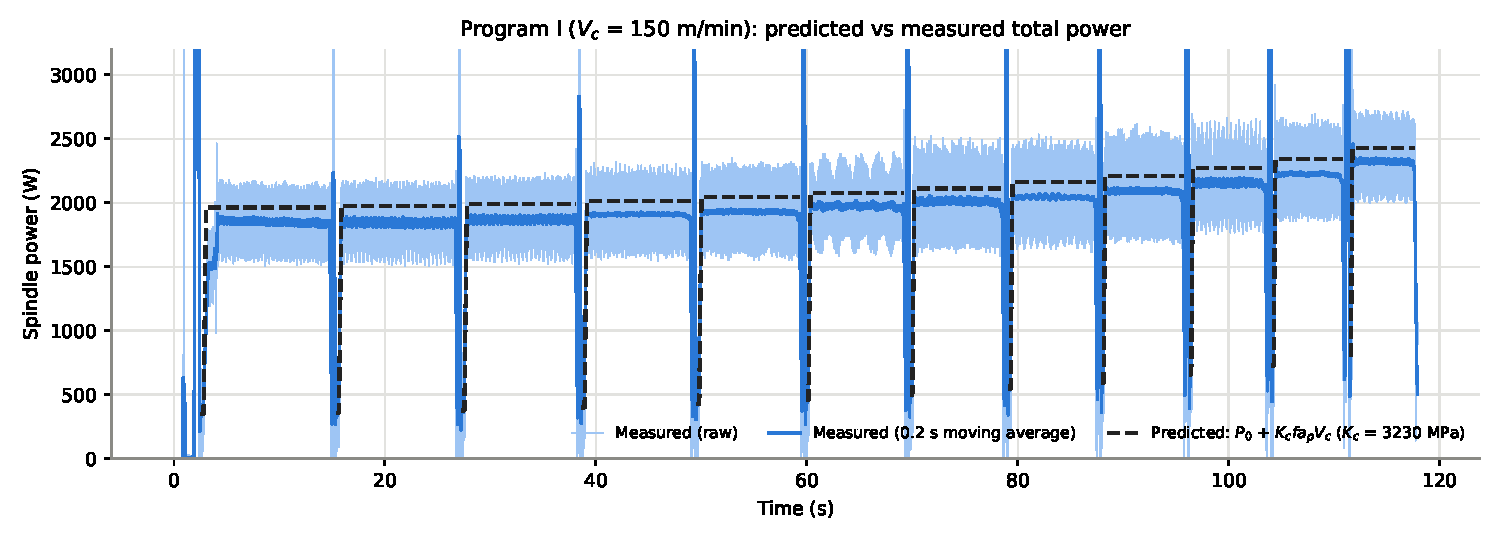
\includegraphics[width=\linewidth]{turning_prediction_vs_measured_vc150.pdf}\\
  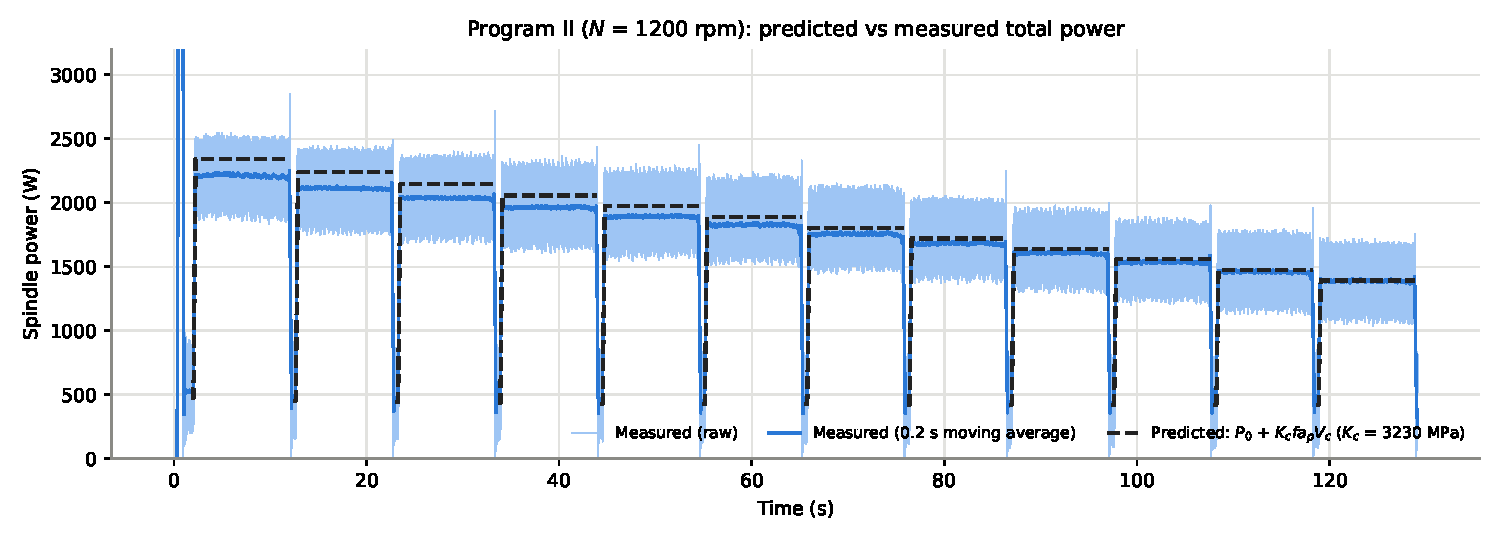
\includegraphics[width=\linewidth]{turning_prediction_vs_measured_n1200.pdf}
  \caption{Predicted total power ($P_0$ + mechanistic $P_c$ with
  $K_c=\KcChapter$~MPa) against the measured power (raw and 0.2~s moving average).}
  \label{fig:pred}
\end{figure}

\subsection{Timings}
Table~\ref{tab:timing} compares, pass by pass, the predicted feed velocity and cutting
time with the measured ones. The measured feed velocity is the slope of the recorded
$Z(t)$. The measured cutting time is the time during which the smoothed power stays
above $P_0+0.5\,P_c$.
\begin{itemize}
  \item The measured $V_f$ equals the predicted $f\,N$ to 0.01~mm/min: in G96 the
        controller applies exactly $N=1000V_c/(\pi X)$.
  \item The cutting time read on the power signal matches $40/V_f$ within
        \SI{0.2}{\percent}. In total, \TcutOne~s are measured against \TcutOnePred~s
        predicted for Program~I, and \TcutTwo~s against \TcutTwoPred~s for Program~II.
        Program~I is faster (total cycle \ToneTot~s against \TtwoTot~s) because the feed
        velocity increases on the small diameters.
  \item The power rises \TonDelayTwo--\TonDelayOne~s after the predicted contact
        $t_0$ and falls about \SI{0.06}{s} after $t_2$. The delay is the same at entry
        and at exit, so it is a lag of the power measurement (drive filtering), not a
        geometric effect. The 10--90\,\% rise time is about \SI{0.1}{s}
        (about 2 revolutions), a little faster than the nose-radius estimate
        $t_1-t_0=r_\varepsilon/V_f\approx\SI{0.2}{s}$ (Fig.~\ref{fig:entry}).
  \item Pass 1 of Program~I is the only exception. The spindle is still accelerating
        when the tool enters: the feed per revolution is respected but $V_f$ is lower
        for about \SI{1.4}{s}, so the contact is late and the power ramp lasts \SI{1}{s}.
\end{itemize}

\begin{table}[H]
\centering\small
\caption{Timing comparison per pass. $\Delta t_0$: time from the start of the pass to
the contact (predicted) and to the power rise (measured). $E$: energy of the cutting run
during the cut; SEC $=E/V_{removed}$.}
\label{tab:timing}
\begin{tabular}{rr rr rr rr r rr}
\toprule
 & $X$ & \multicolumn{2}{c}{$V_f$ (mm/min)} & \multicolumn{2}{c}{$\Delta t_0$ (s)} &
 \multicolumn{2}{c}{$T_{cut}$ (s)} & rise & $E$ & SEC \\
 \cmidrule(lr){3-4}\cmidrule(lr){5-6}\cmidrule(lr){7-8}
pass & (mm) & pred. & meas. & pred. & meas. & pred. & meas. & (s) & (kJ) & (J/mm$^3$)\\
\midrule
\multicolumn{11}{l}{\emph{Program I -- $V_c=150$ m/min}}\\
\rowsinput{../results/timing_vc150_rows.tex}
\midrule
\multicolumn{11}{l}{\emph{Program II -- $N=1200$ rpm}}\\
\rowsinput{../results/timing_n1200_rows.tex}
\bottomrule
\end{tabular}
\end{table}

\begin{figure}[H]
  \centering
  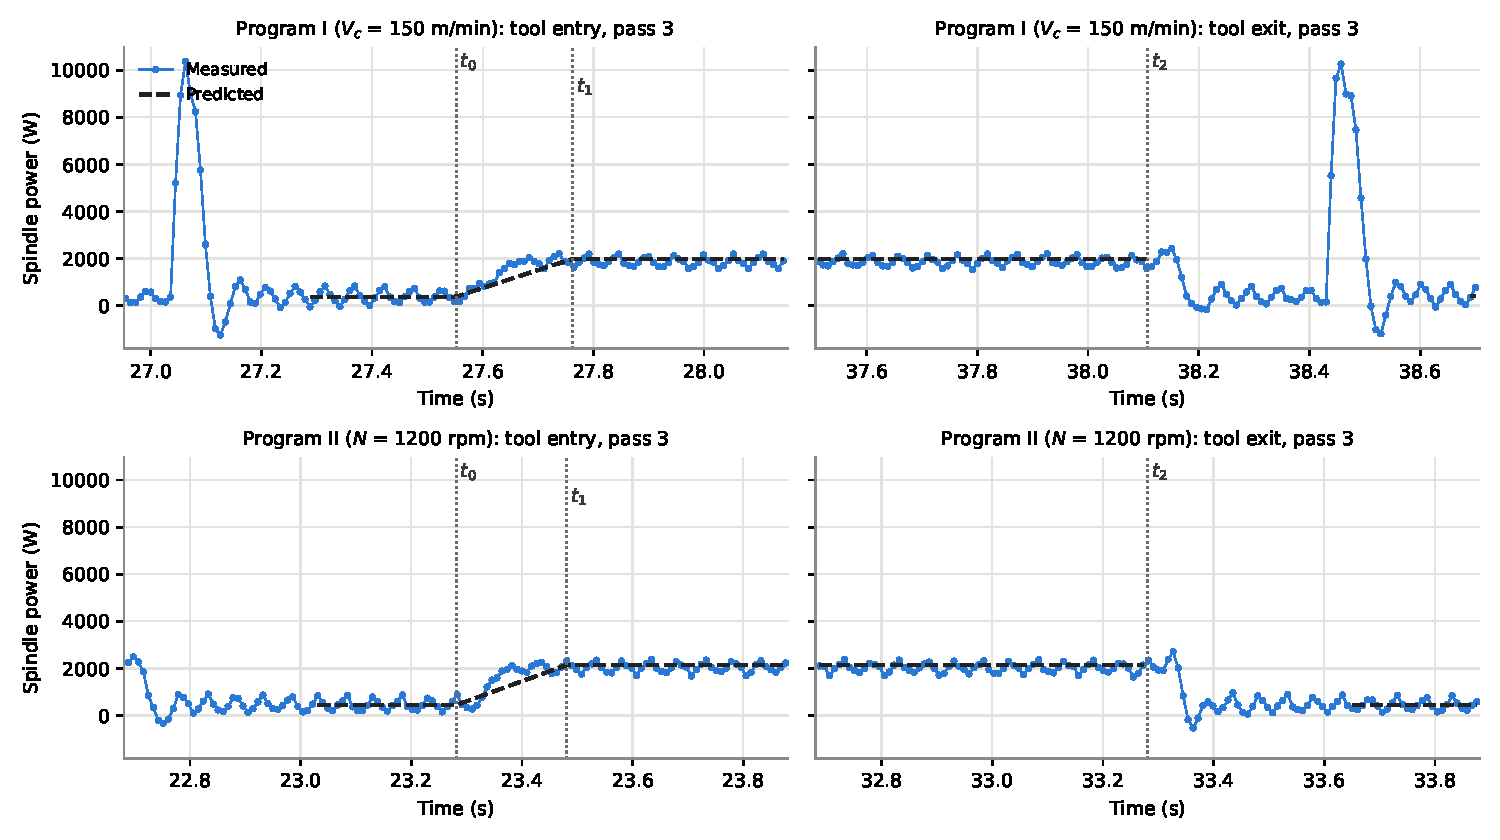
\includegraphics[width=\linewidth]{turning_entry_exit.pdf}
  \caption{Tool entry and exit (pass 3): measured samples and prediction.}
  \label{fig:entry}
\end{figure}

\subsection{Curve profile: conclusions}
\begin{figure}[H]
  \centering
  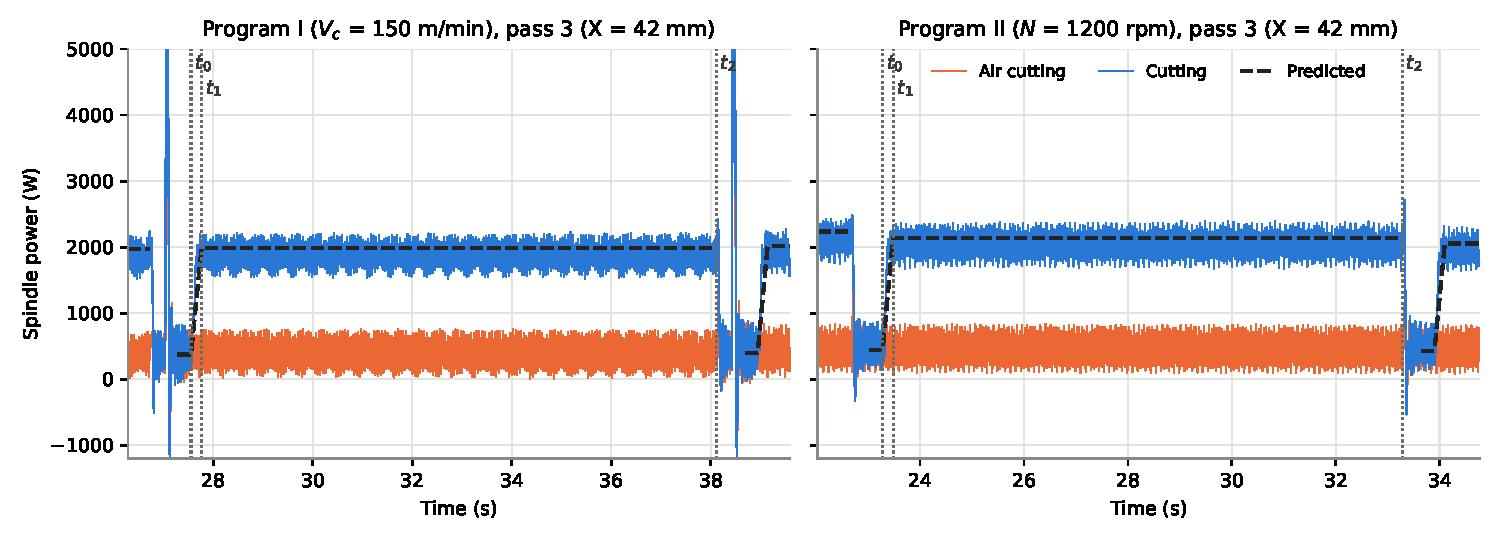
\includegraphics[width=\linewidth]{turning_zoom_pass.pdf}
  \caption{Pass 3 of both programs: cutting run, air-cutting run (re-aligned on the
  same pass) and prediction.}
  \label{fig:zoom}
\end{figure}

\begin{enumerate}
  \item \textbf{Plateaus.} During each pass the power is a flat plateau, as predicted:
        $f$, $a_p$ and $V_c$ do not change along $Z$. The plateau level is $P_0+P_c$.
        The recorded curve is the sum of the mechanistic cutting power and of the power
        needed to keep the spindle rotating.
  \item \textbf{Program I.} $P_c$ is constant (\PcOneMean~W measured), but the total
        power \emph{increases} pass after pass (1851 to 2323~W) because $P_0$ grows with
        the spindle speed (\PzeroOneFirst\ to \PzeroOneLast~W). The rise comes from the
        spindle, not from the cut. The plateaus get shorter because $V_f=fN$ increases.
  \item \textbf{Program II.} $P_0$ is almost constant and $P_c\propto V_c\propto X$
        decreases linearly (\PcTwoFirst\ to \PcTwoLast~W), so the total power
        \emph{decreases} pass after pass, with plateaus of constant length.
  \item \textbf{Level of the prediction.} With the constant $K_c=\KcChapter$~MPa, the
        predicted cutting power is \PcErrOneMin--\PcErrOneMax\,\% too high in
        Program~I. In Program~II the error is \PcErrTwoMax\,\% on the first passes (high
        $V_c$) and falls to \PcErrTwoMin\,\% on the last one, the pass on which $K_c$ was
        obtained. The
        error grows with the cutting speed: $K_c$ is not exactly constant but decreases
        when $V_c$ increases (Section~\ref{sec:kc}). The \emph{shape} and the
        \emph{timings} of the curves are reproduced exactly.
  \item \textbf{Peaks between passes.} In Program~I each plunge to a smaller diameter
        makes the G96 controller accelerate the spindle, which gives peaks of about
        \SI{10}{kW} (inertial power $J\omega\dot\omega$). They are preceded by negative
        values when the tool retracts in X and the spindle is braked (regenerative
        drive). In Program~II the speed never changes, so the only large peak is the
        initial spindle start. These transients are outside the cutting model but
        consume energy.
  \item \textbf{Ripple.} The raw signal oscillates by $\pm$\SIrange{200}{300}{W} around
        the plateau, with and without cutting, at the rotation frequency $N/60$
        (20.0~Hz at 1200~rpm, Fig.~\ref{fig:spectrum}). It is a once-per-revolution
        effect of the rotating assembly (unbalance or eccentricity of chuck and bar), not
        a cutting phenomenon, and it averages out over the steady-state window.
  \item \textbf{Energy.} Despite the different profiles, the energy spent during the
        cut is almost the same in the two programs: \EOne~kJ against \ETwo~kJ in
        total, of which \ECutOne~kJ against \ECutTwo~kJ for cutting. The cutting energy
        per unit volume equals $K_c$ (SEC$_{cut}$ = \SECcutOne\ and \SECcutTwo~J/mm$^3$,
        i.e.\ about \SI{3000}{MPa}) and does not depend on the strategy; the difference
        lies in the non-productive spindle energy.
\end{enumerate}

\begin{figure}[H]
  \centering
  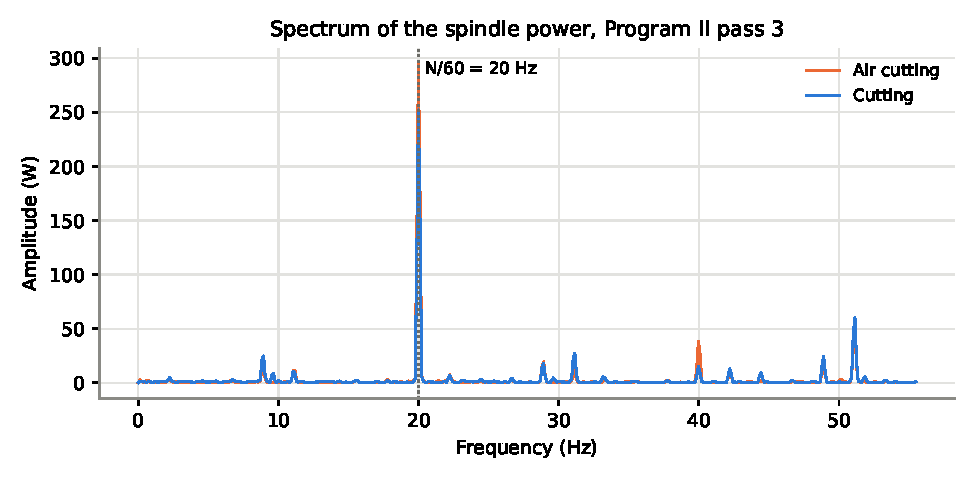
\includegraphics[width=0.65\linewidth]{turning_power_spectrum.pdf}
  \caption{Amplitude spectrum of the spindle power in steady state (Program II, pass
  3): the ripple is at the rotation frequency $N/60$.}
  \label{fig:spectrum}
\end{figure}

% ===========================================================================
\section{Point 3 -- Specific cutting pressure from the recorded power}\label{sec:kc}
% ===========================================================================
\subsection{Method}
For every pass the code:
\begin{enumerate}
  \item finds the feed motions from the derivative of the programmed $Z$ (feed between
        30 and 1000~mm/min). This pairs the cutting run and the air-cutting run pass by
        pass, even though the two runs are shifted in time;
  \item takes the \emph{steady-state window} $-3\geq Z \geq -37$~mm: the tool is fully
        engaged and far from the entry/exit transients and from the acceleration peaks.
        The window covers tens of revolutions, so the once-per-revolution ripple averages
        out;
  \item computes $P_{tot}$, the mean power of the cutting run, and $P_0$, the mean
        power of the air-cutting run in the same window (spindle power without cutting,
        same speed, same axis motions);
  \item computes the cutting power and the specific cutting pressure (chapter Eqs.~5--6):
\end{enumerate}
\begin{equation}
  P_c = P_{tot}-P_0,\qquad
  F_c = \frac{P_c}{V_c},\qquad
  K_c = \frac{P_c}{f\,a_p\,V_c} .
\end{equation}
\begin{lstlisting}[language=Python]
p_tot, _ = steady_state_mean(cut, pc.i_start, pc.i_end, Z_HI, Z_LO)  # cutting run
p_air, _ = steady_state_mean(air, pa.i_start, pa.i_end, Z_HI, Z_LO)  # air cutting
p_cut = p_tot - p_air
Kc = kc_turning(p_cut, F, AP, Vc)            # = p_cut / (F*AP*Vc/60)
\end{lstlisting}

\subsection{Results}
\begin{table}[H]
\centering\small
\caption{Program I ($V_c=150$ m/min): steady-state powers (W), cutting force (N) and
specific cutting pressure (MPa), compared with Table~2 of the chapter.}
\label{tab:p1}
\begin{tabular}{rrrr rrr r rr}
\toprule
pass & $X$ & $N$ & $V_c$ & $P_{tot}$ & $P_0$ & $P_c$ & $F_c$ & $K_c$ & $K_c$ chapter\\
\midrule
\rowsinput{../results/turning_vc150_rows.tex}
\bottomrule
\end{tabular}
\end{table}

\begin{table}[H]
\centering\small
\caption{Program II ($N=1200$ rpm): same quantities as Table~\ref{tab:p1}. The last
row is the reference used for drilling.}
\label{tab:p2}
\begin{tabular}{rrrr rrr r rr}
\toprule
pass & $X$ & $N$ & $V_c$ & $P_{tot}$ & $P_0$ & $P_c$ & $F_c$ & $K_c$ & $K_c$ chapter\\
\midrule
\rowsinput{../results/turning_n1200_rows.tex}
\bottomrule
\end{tabular}
\end{table}

\begin{figure}[H]
  \centering
  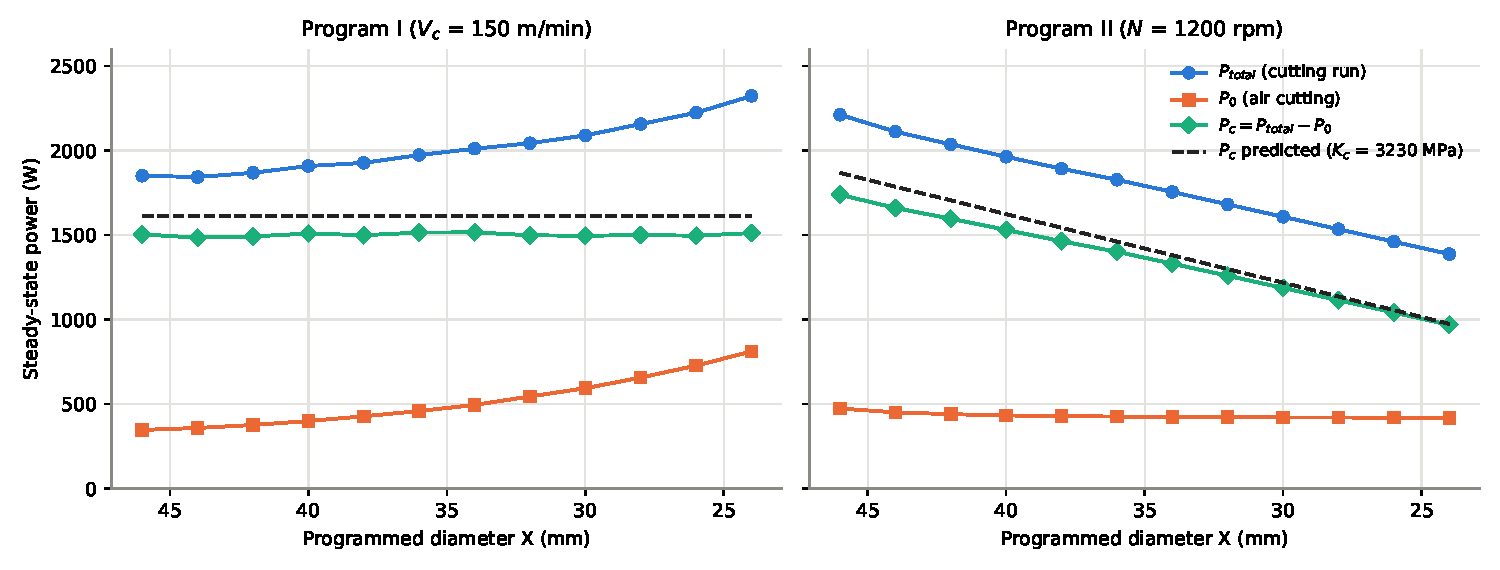
\includegraphics[width=\linewidth]{turning_steady_state_power.pdf}
  \caption{Steady-state powers per pass: total, without cutting, cutting power
  (identified and predicted at point 1).}
  \label{fig:ss}
\end{figure}

\begin{figure}[H]
  \centering
  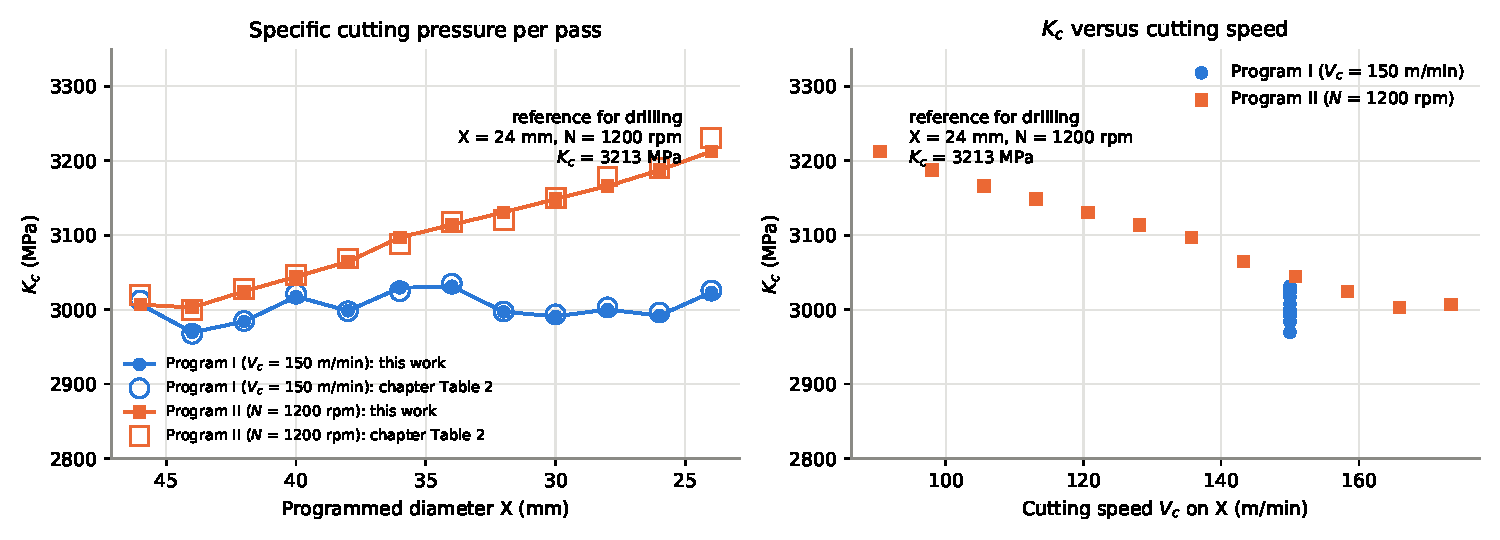
\includegraphics[width=\linewidth]{turning_kc.pdf}
  \caption{Specific cutting pressure identified on every pass, compared with the chapter.}
  \label{fig:kc}
\end{figure}

\paragraph{Discussion.}
\begin{itemize}
  \item The values reproduce Table~2 of the chapter within \KcDevMax\,\%. Program~I:
        $K_c=\KcOneMean\pm\KcOneStd$~MPa. Program~II: $K_c$ from \KcTwoMin\ to
        \KcTwoMax~MPa.
  \item \textbf{Reference value for point 4} (smallest diameter, constant spindle
        speed, $X=\SI{24}{mm}$, $N=\SI{1200}{rpm}$): $P_c=\PcRef$~W, $F_c=\FcRef$~N,
        $V_c=\VcRef$~m/min, $K_c=\KcRef$~MPa. The chapter gives 3230.3~MPa because it
        uses the rounded speed $V_c=\SI{90}{m/min}$; with the exact speed $\pi\cdot 24
        \cdot 1200/1000=\SI{90.48}{m/min}$ the same power gives \KcRef~MPa.
  \item In Program~II, $K_c$ increases when $V_c$ decreases (from 173 to 90 m/min,
        Fig.~\ref{fig:kc} right). This is the known decrease of the cutting force with
        the cutting speed at moderate speeds (softening of the shear zone, see the
        ``Experiments'' slide). In Program~I, where $V_c$ is constant, $K_c$ is constant
        too. A constant-$K_c$ model is therefore exact only at the speed where $K_c$ was
        measured, which explains the deviations found at point 2.
  \item $P_0$ follows a quadratic law of the speed in Program~I,
        $P_0\approx\IdleA+\IdleB\,N+\IdleC\cdot10^{-4}N^2$ (W, rpm), Fig.~\ref{fig:idle}.
        In Program~II, at constant 1200~rpm, $P_0$ decreases from \PzeroTwoFirst\ to
        \PzeroTwoLast~W and tends to the value \PzeroFitTwelve~W of the Program~I fit:
        the spindle is warming up (viscosity of the bearing lubricant). Since $P_0$ is
        measured in a separate run, a different thermal state between the cutting and
        air-cutting runs is the main uncertainty of the method: $\pm$\SI{30}{W} on $P_0$
        gives about $\pm$\SI{100}{MPa} on $K_c$ at 90 m/min.
\end{itemize}

\begin{figure}[H]
  \centering
  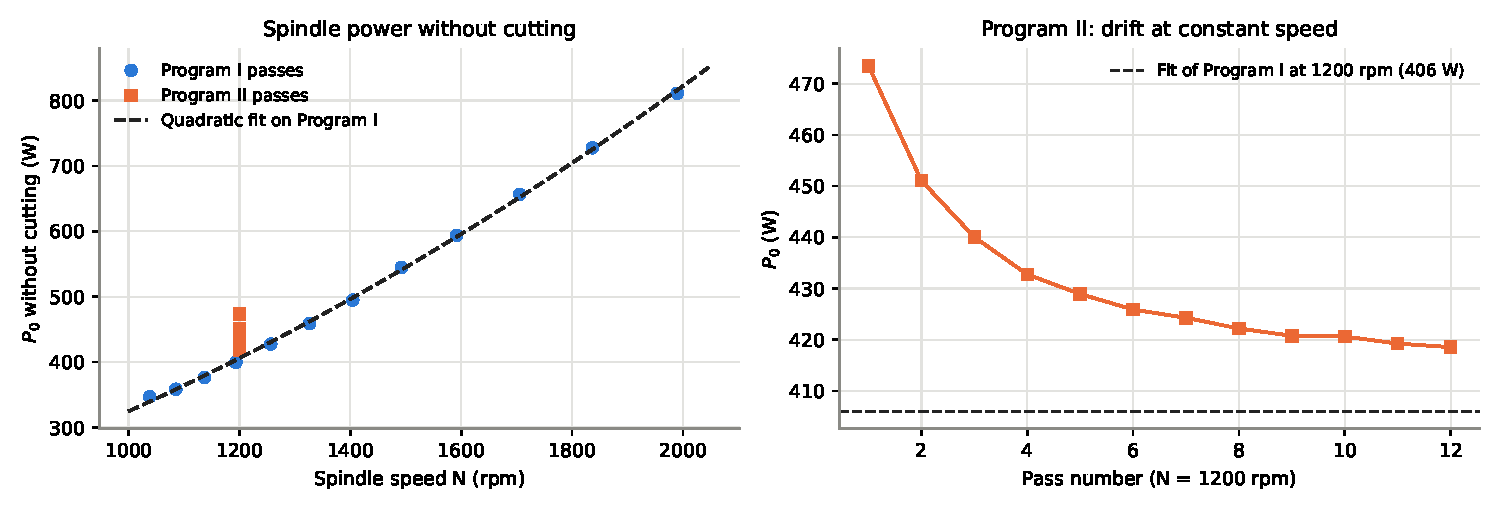
\includegraphics[width=\linewidth]{turning_idle_power.pdf}
  \caption{Spindle power without cutting: dependence on the spindle speed and thermal
  drift at constant speed.}
  \label{fig:idle}
\end{figure}

\subsection{Minimum and maximum values}\label{sec:minmax}
The recorded power is noisy: around each plateau it oscillates once per revolution
(Fig.~\ref{fig:spectrum}). Besides the mean, the minimum and maximum of the power were
therefore taken in the same steady-state window, for the cutting run and for the
air-cutting run. To avoid that a single outlier sample sets the value, the minimum and
maximum are the 1\,\% and 99\,\% percentiles of the samples of the window. The cutting
power and the specific cutting pressure are then computed from the minima and from the
maxima:
\begin{equation}
  P_{c}^{min} = P_{tot}^{min}-P_0^{min},\qquad P_{c}^{max} = P_{tot}^{max}-P_0^{max},\qquad
  K_c^{min,max} = \frac{P_c^{min,max}}{f\,a_p\,V_c}.
\end{equation}
The minimum of the cutting run is paired with the minimum of the air-cutting run, and the
maximum with the maximum, because the oscillation comes from the rotation and is
present in both runs.

\begin{table}[H]
\centering\small
\caption{Minimum and maximum steady-state powers (W) and the resulting specific cutting
pressure (MPa), compared with the value from the mean powers.}
\label{tab:range}
\begin{tabular}{rr rr rr rr rrr}
\toprule
 & $X$ & \multicolumn{2}{c}{$P_{tot}$} & \multicolumn{2}{c}{$P_0$} &
 \multicolumn{2}{c}{$P_c$} & \multicolumn{3}{c}{$K_c$}\\
 \cmidrule(lr){3-4}\cmidrule(lr){5-6}\cmidrule(lr){7-8}\cmidrule(lr){9-11}
pass & (mm) & min & max & min & max & from min & from max & from min & mean & from max\\
\midrule
\multicolumn{11}{l}{\emph{Program I -- $V_c=150$ m/min}}\\
\rowsinput{../results/range_vc150_rows.tex}
\midrule
\multicolumn{11}{l}{\emph{Program II -- $N=1200$ rpm}}\\
\rowsinput{../results/range_n1200_rows.tex}
\bottomrule
\end{tabular}
\end{table}

\begin{figure}[H]
  \centering
  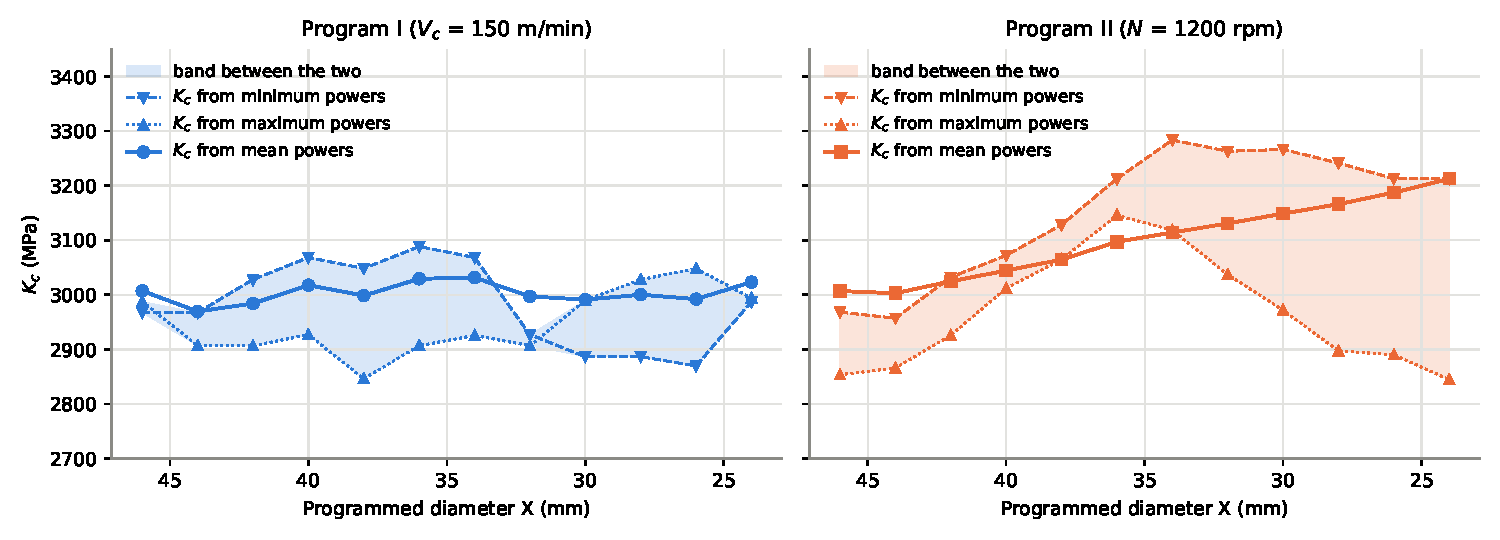
\includegraphics[width=\linewidth]{turning_kc_range.pdf}
  \caption{Specific cutting pressure from the mean, minimum and maximum powers.}
  \label{fig:kcrange}
\end{figure}

\begin{itemize}
  \item Within a pass the power swings by about \SwingCut~W with cutting and
        \SwingAir~W without cutting, i.e.\ by the same amount. The oscillation is not
        produced by the cut but by the rotating assembly, and it is simply added to the
        cutting power.
  \item For this reason $P_c$ from the minima and $P_c$ from the maxima stay close to
        $P_c$ from the means. All the $K_c$ values fall between \KcRangeMin\ and
        \KcRangeMax~MPa, at most \DevMinMax\,\% from the value obtained from the means.
        The band is at most \BandOne~MPa wide in Program~I and \BandTwo~MPa in
        Program~II. In both cases it is wider than the change of $K_c$ from one pass to
        the next.
  \item On the reference pass ($X=24$~mm, $N=1200$~rpm), $K_c$ is \KcRefMin~MPa from
        the minima, \KcRef~MPa from the means and \KcRefMax~MPa from the maxima.
  \item Pairing the values the other way round ($P_{tot}^{min}-P_0^{max}$ and
        $P_{tot}^{max}-P_0^{min}$) would give, on the same pass, $K_c$ between
        \KcCrossLo\ and \KcCrossHi~MPa. This range has no physical meaning: it only
        adds up the two oscillations, which happen together.
  \item The minimum and maximum come from a few samples at the extremes of the
        oscillation, while the mean uses all the samples of the window. The mean is
        therefore the most robust estimate, and it is the value used for the drilling
        prediction.
\end{itemize}

% ===========================================================================
\section{Point 4 -- Prediction of the drilling sequence}
% ===========================================================================
\subsection{Data and model}
The specific cutting pressure and the cutting speed of point~3 are used:
$K_c=\DrKc$~MPa, $K_f=0.4\,K_c=\DrKf$~MPa and $V_c=\DrVc$~m/min (peripheral speed of
the drill). The sequence is:
\begin{itemize}
  \item pre-drilling $\varnothing$\SI{5}{mm}, point angle \ang{120}, machining length
        \SI{10}{mm}, $f=\SI{0.2}{mm/rev}$: $N=\DrFiveN$~rpm, $V_f=\DrFiveVf$~mm/min;
  \item drilling $\varnothing$\SI{13}{mm} in the same position, point angle \ang{120},
        machining length \SI{20}{mm}, $f=\SI{0.2}{mm/rev}$: $N=\DrThirteenN$~rpm,
        $V_f=\DrThirteenVf$~mm/min.
\end{itemize}
The machining length is taken as the depth of the drill tip below the part surface at
the end of the feed. The tool starts \SI{1}{mm} above the surface; times are measured
from the start of the feed.

Following the course slides (``Machining forces in drilling''), each of the two lips
cuts with a feed per tooth $f_z=f/2$ and a cutting speed that grows linearly with the
radius, $V_c(r)=2\pi rN/1000$ (Fig.~\ref{fig:vc}). Each lip is divided into elements
$dr$:
\begin{equation}
  dF_c = K_c\, f_z\, dr,\qquad dF_f = K_f\, f_z\, dr,\qquad dP_c = dF_c\,V_c(r),
\end{equation}
summed over the elements that are in the material, for both lips. With the drill tip at
depth $z$, an element at radius $r$ sits at $z-r\cot 60^\circ$ and cuts if it is below
the surface and not inside the pilot hole. On the full lip this gives the formulas of
the slides:
\begin{equation}
  P_c = 2\,K_c\,\frac{D}{2}\,\frac{f}{2}\,\frac{V_{c}}{2} = K_c\,\frac{\pi D^2}{4} f N,\qquad
  F_f = K_f\,\frac{D}{2}\,f,\qquad M_c=\frac{P_c}{\omega}=K_c\,\frac{D^2 f}{8}.
\end{equation}
When enlarging a pilot hole of diameter $d$ the lips only cut the annulus
$d/2\le r\le D/2$:
\begin{equation}
  P_c = K_c\,\frac{\pi (D^2-d^2)}{4} f N,\qquad F_f = K_f\,\frac{D-d}{2}\,f .
\end{equation}
The chisel edge is neglected (it adds thrust force but little power), and so is the
spindle power without cutting: $P_0(N)$ was only measured up to 2000~rpm, and
extrapolating it to the 5760~rpm of the $\varnothing$5 drill would not be reliable.

\begin{figure}[H]
  \centering
  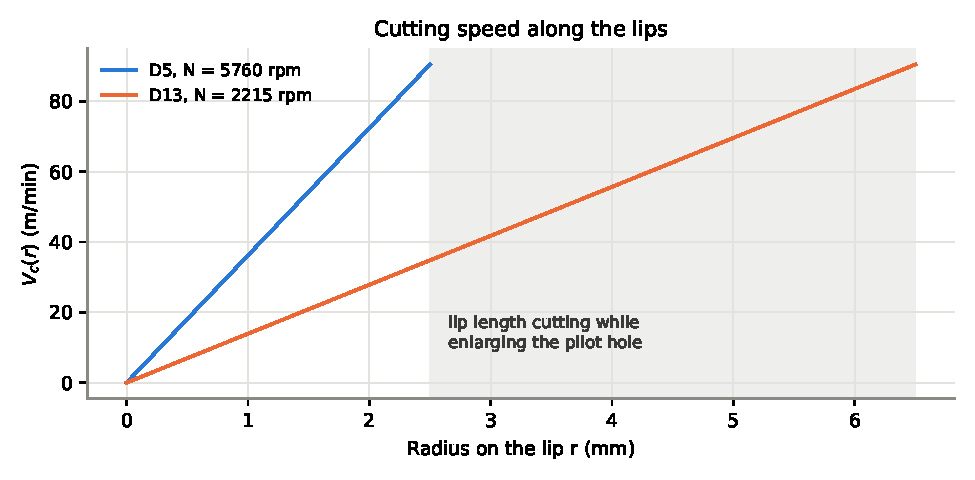
\includegraphics[width=0.7\linewidth]{drilling_edge_speed.pdf}
  \caption{Cutting speed along the lips. Shaded: part of the $\varnothing$13 lip that
  cuts while the pilot hole is being enlarged.}
  \label{fig:vc}
\end{figure}

\subsection{Characteristic instants}
\textbf{Pre-drilling $\varnothing$5:}
\begin{itemize}
  \item $t_0=\DrFiveTZero$~s: the tip touches the part ($z=0$);
  \item $t_1=\DrFiveTOne$~s: the conical point (height $2.5/\tan 60^\circ=\DrFiveZOne$~mm)
        is fully inside the material;
  \item $t_2=\DrFiveTTwo$~s: end of the machining length ($z=\SI{10}{mm}$).
\end{itemize}
\textbf{Drilling $\varnothing$13 inside the pilot hole:}
\begin{itemize}
  \item $t_0=\DrThirteenTZero$~s: the lips touch the edge of the pilot hole, at
        $r=\SI{2.5}{mm}$, when the tip is at $z=\DrThirteenZZero$~mm. Before that, the
        tip moves in the empty pilot hole;
  \item $t_1=\DrThirteenTOne$~s: the whole annulus $2.5\le r\le 6.5$~mm is engaged
        ($z=\DrThirteenZOne$~mm), and the hole is being enlarged;
  \item $t_2=\DrThirteenTTwo$~s: the tip reaches the bottom of the pilot hole
        ($z=\SI{10}{mm}$). The bottom of the pilot hole is a cone with the same
        \ang{120} angle as the drill, so the inner part of the lips ($r<2.5$~mm) engages
        \emph{all at once}: power, force and torque step up. In practice the chisel edge
        also starts working here, which makes the thrust step even larger;
  \item $t_3=\DrThirteenTThree$~s: end of the machining length ($z=\SI{20}{mm}$), full
        diameter drilling between $t_2$ and $t_3$.
\end{itemize}

\subsection{Predicted curves}
\begin{table}[H]
\centering\small
\caption{Steady values of each phase of the drilling sequence ($K_c=\DrKc$~MPa,
$K_f=\DrKf$~MPa, $V_c=\DrVc$~m/min).}
\label{tab:drill}
\begin{tabular}{llrrrrr}
\toprule
drill & phase & cutting radii (mm) & $F_f$ (N) & $P_c$ (W) & $M_c$ (N\,m) & $P_f$ (W)\\
\midrule
\rowsinput{../results/drilling_rows.tex}
\bottomrule
\end{tabular}
\end{table}

\begin{figure}[H]
  \centering
  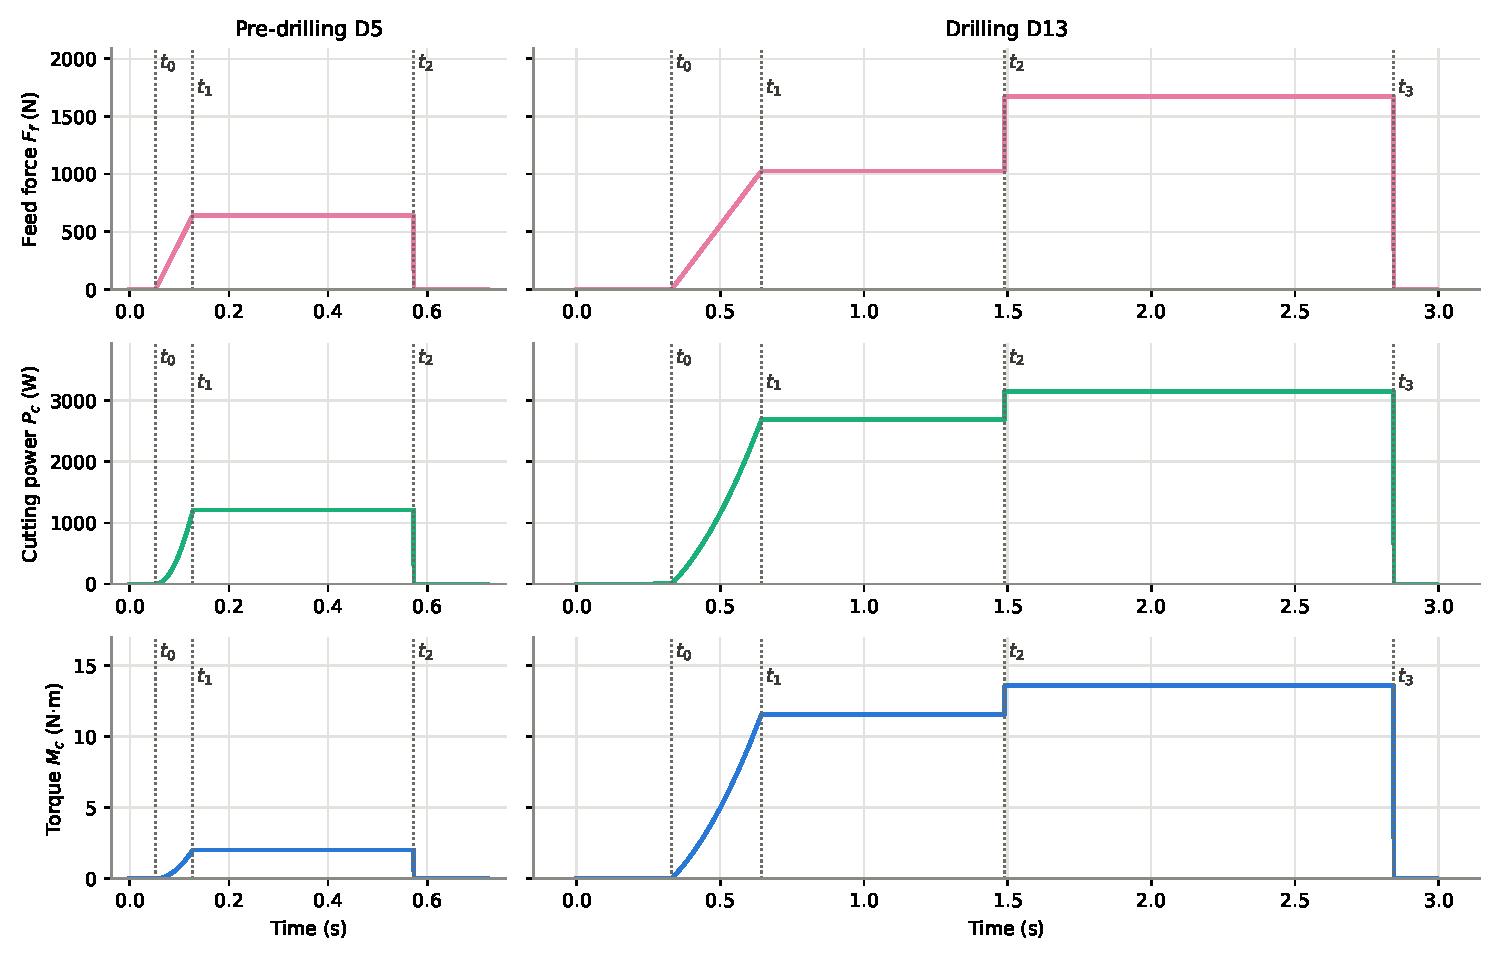
\includegraphics[width=\linewidth]{drilling_sequence.pdf}
  \caption{Predicted feed force, cutting power and torque of the two operations, on the
  same vertical scales.}
  \label{fig:drillseq}
\end{figure}

\paragraph{Curve profile.}
\begin{itemize}
  \item \textbf{Entry ($t_0\to t_1$).} The engaged lip length grows linearly with the
        penetration, so the feed force grows \emph{linearly} in time. Power and torque
        also depend on the radius of the engaged elements ($V_c\propto r$), so they grow
        \emph{quadratically} for the $\varnothing$5 drill. For the $\varnothing$13 drill
        they start from $r=2.5$~mm, where $V_c$ is already 35~m/min, so the curve is
        closer to a straight line.
  \item \textbf{Pilot hole.} The pilot hole cuts the thrust force of the
        $\varnothing$13 drill by 38\,\% during the enlargement (1028 against
        1671~N). The cutting power drops by only 15\,\% (2683 against 3149~W) because the
        removed core is the part of the lip with the lowest cutting speed. This is why
        pilot holes are used to reduce the axial load.
  \item \textbf{Comparison of the two drills.} With the same $V_c$ and the same $f$,
        the $\varnothing$13 drill turns 2.6 times slower and $V_f$ is 2.6 times lower.
        Its power is 2.6 times higher (proportional to $D$) and its torque 6.8 times
        higher (proportional to $D^2$).
  \item \textbf{Energy.} The cutting energy is $E=\int P_c\,dt=K_c\,V_{removed}$:
        \DrFiveE~J for the pre-drilling and \DrThirteenE~J for the drilling.
  \item \textbf{Limits.} $K_c$ was measured in turning with an uncut chip thickness
        $h=f\sin\kappa_r\approx\SI{0.2}{mm}$. In drilling $h=f_z\sin 60^\circ\approx
        \SI{0.087}{mm}$, and the speed varies from 0 to 90~m/min along the lip. Both
        effects (size effect and low speed near the centre, Fig.~\ref{fig:kc}) would
        increase the real $K_c$, so the predicted curves are a lower bound. The chisel
        edge, the friction of the margins and the chip evacuation in the
        \SI{20}{mm}-deep hole (see the torque curves of Davim in the slides) are not
        modelled either. The total power read by the machine would also include
        $P_0(N)$.
\end{itemize}

% ===========================================================================
\section{Conclusions}
% ===========================================================================
\begin{itemize}
  \item With $K_c=\KcChapter$~MPa (chapter, smallest diameter) the mechanistic model
        predicts the timings of every pass within \SI{0.2}{\percent}. It overestimates
        the cutting power by up to about 9\,\% at high cutting speed, because $K_c$
        decreases when $V_c$ increases.
  \item The recorded total power is the sum of a spindle term $P_0(N)$ and of the
        cutting term: in Program~I the total power rises because of the spindle, in
        Program~II it falls because of the cut. Acceleration peaks of about \SI{10}{kW}
        appear only when the spindle speed changes (Program~I). The power signal lags
        the position by about \SI{0.07}{s}.
  \item The Python code separates the steady-state cutting power from the spindle power
        without cutting and finds $K_c$ for every pass within \KcDevMax\,\% of the
        chapter. On the smallest diameter at constant spindle speed,
        $K_c=\KcRef$~MPa at $V_c=\VcRef$~m/min. Computed from the minimum and maximum
        powers instead of the means, $K_c$ stays between \KcRangeMin\ and
        \KcRangeMax~MPa, because the power oscillation is the same with and without
        cutting.
  \item Drilling sequence: the $\varnothing$5 pre-drilling needs about 1.2~kW, 643~N and
        2.0~N\,m. The $\varnothing$13 drilling needs 2.7~kW and 1.0~kN while it enlarges
        the pilot hole, then steps up to 3.1~kW, 1.7~kN and 13.6~N\,m when the tip
        reaches the bottom of the pilot hole at $t_2$.
\end{itemize}

\appendix
\section{Python code: where to find it and how to run it}\label{app:code}
\paragraph{Repository.} The code and the data are in the folder \texttt{Assigment1} of
\begin{center}
\url{https://github.com/DanTrisi/MASSMA_1_TOLOSA/tree/master/Assigment1}
\end{center}
\begin{lstlisting}
run_all.py                 # runs the whole analysis (turning first, then drilling)
src/machining.py           # models (turning, drilling), CSV reader,
                           # pass detection, steady-state mean / min / max
src/turning_analysis.py    # points 1-3: prediction, timings, P0, Pc, Fc, Kc
src/drilling_analysis.py   # point 4: drilling sequence D5 + D13
src/plotstyle.py           # common style of the figures
data/                      # the four CSV traces of the chapter_2025 repository
plot/                      # figures of this report, as produced by the code
results/                   # tables of results, as produced by the code
\end{lstlisting}
The four CSV files in \texttt{data/} are an unmodified copy of the traces published in
\texttt{github.com/annacarlaaraujo/chapter\_2025}. If a file is missing, the code stops
and says which one.

\paragraph{Requirements.} Python 3.10 or newer with \texttt{numpy} ($\geq 2.0$),
\texttt{pandas} and \texttt{matplotlib}:
\begin{lstlisting}
pip install numpy pandas matplotlib
\end{lstlisting}

\paragraph{Run.} Download the repository (\emph{Code} $\rightarrow$ \emph{Download ZIP}
on GitHub, or \texttt{git clone}) and run the analysis from the \texttt{Assigment1}
folder:
\begin{lstlisting}
git clone https://github.com/DanTrisi/MASSMA_1_TOLOSA.git
cd MASSMA_1_TOLOSA/Assigment1
python run_all.py
\end{lstlisting}
The turning analysis must run before the drilling one, because the drilling prediction
uses the specific cutting pressure identified in turning; \texttt{run\_all.py} keeps this
order. The two scripts can also be run one at a time
(\texttt{python src/turning\_analysis.py}, then \texttt{python src/drilling\_analysis.py}).

\paragraph{Output.} The main results (powers, $K_c$ per pass, drilling values and
instants) are printed in the terminal. The figures of this report are saved (or
overwritten) in \texttt{plot/} (PDF and PNG). The tables of results are saved in
\texttt{results/},
including \texttt{kc\_reference.csv}, which carries the reference $K_c$ and $V_c$
from the turning analysis to the drilling prediction.

\end{document}
